\documentclass[10pt, compress]{beamer}
\includeonlyframes{current}

\setbeamerfont{itemize/enumerate subbody}{size=\normalsize} 

\usetheme{m}

\usepackage{booktabs}
\usepackage[scale=2]{ccicons}
\usepackage{minted}
\usepackage{graphicx}
\usepackage{subfig}
\usepackage[export]{adjustbox}
\usepackage{physics}
\usepackage{amsmath}

\usepackage{appendixnumberbeamer}

\usepackage[overlay,absolute]{textpos}

\usepackage{layout}
\usepackage{printlen}
\usepackage{tcolorbox}

\usepackage[none]{hyphenat}

\usepackage{animate}

\usepackage{tikz}
\usetikzlibrary{arrows,positioning,shapes,decorations.markings}



%\pgfdeclareimage[height=\paperheight,width=\paperwidth,keepaspectratio]{myimage}{figs/16Cygni.png}
%\usebackgroundtemplate{\tikz\node[opacity=0.01,inner sep=0] {\pgfuseimage{myimage}};}
%\usebackgroundtemplate{%
%\tikz\node[opacity=0.05] {\includegraphics[height=\paperheight,width=\paperwidth]{figs/16Cygni.png}};}


%%%% TESSERACT %%%%%%%%%%%%%%%%%%%%%%%%
\def\mycommand{low $\alpha$\gdef\mycommand{high $\alpha$}}
\newcommand{\getlabel}[2] {
    \ifnum#1<2
        \ifnum#2<1
            low $M$
        \else
            high $M$
        \fi
    \else
        \ifnum#1=2
            \ifnum#2<3
                low $Y$
            \else
                high $Y$
            \fi
        \else
            \ifnum#1=3
                \ifnum\ifnum#2=3 1\else\ifnum#2=6 1\else 0\fi\fi=1
                    low $Z$
                \else
                    high $Z$
                \fi
            \else
                \ifnum\ifnum#2=4 1\else\ifnum#2=7 1\else\ifnum#2=8 1\else\ifnum#2=9 1\else 0\fi\fi\fi\fi=1
                    \ifnum#2=7
                        \expandafter\mycommand
                    \else
                        low $\alpha$
                    \fi
                \else
                    high $\alpha$
                \fi
            \fi
        \fi
    \fi
}

% a little support for all the keys
\def\hyperset{\pgfqkeys{/tikz/hyper}}
\tikzset{hypher/.code=\hyperset{#1}}

% Dimension setup
\hyperset{
  set color/.code 2 args={\colorlet{tikz@hyper@dimen@#1}{#2}},
  set color={0}{black},%{black},
  set color={1}{black},%{blue!50!black},
  set color={4}{yellow!40!black},%{red},
  set color={3}{blue!50!black},%{green},
  set color={2}{red!80!black}}%{yellow!80!black}}
\hyperset{
  set dimens/.style args={#1:(#2)}{
    dimen #1/.style={/tikz/shift={(#2)}}},
  set dimens=0:(0:0),
  set dimens=1:(right:1.2),%.4),
  set dimens=2:(up:1.1),%.05),
  set dimens=3:(30:.6),%.75),
  set dimens=4:(180+70:.5),%.5),
  every hyper node/.style 2 args={%
    shape=circle,
    inner sep=+0pt,
    %fill,
    fill=black,
    draw,
    minimum size=+3pt,
    %color=tikz@hyper@dimen@#1,
    label={[hyper/label #1/.try, hyper/dimen #1 style/.try] \getlabel{#1}{#2}}
  },
  every hyper edge/.style={draw},
  every hyper shift edge/.style={<->,dashed,line width=.25mm,tikz@hyper@dimen@#1!100},
  every normal hyper edge/.style={<->,dashed,line width=.25mm,tikz@hyper@dimen@#1!100},
}
\newcommand*{\hyper}[1]{% #3 = max level
  \def\currentTransform{}
  \node[hyper/every hyper node/.try={0}{0}, hyper/dimen 0 node/.try] (0-0) {};
  \hyperhyper{0}{0}{#1}}
\newcommand*{\hyperhyper}[3]{% #1 = current level
                             % #2 = current number
                             % #3 = maxlevel
  \foreach \dimension in {#3,...,\the\numexpr#1+1\relax} {
    \edef\newNumber{\the\numexpr#2+\dimension\relax}
    \node[hyper/every hyper node/.try={\dimension}{\newNumber}, hyper/dimen \dimension node/.try, hyper/dimen \dimension\space style/.try] at ([hyper/dimen \dimension] #1-#2) (\dimension-\newNumber) {};
    \path (#1-#2) edge[hyper/every hyper edge/.try=\dimension, hyper/every hyper shift edge/.try=\dimension, hyper/dimen \dimension\space style/.try] (\dimension-\newNumber);
    \ifnum\newNumber>\dimension\relax
      \foreach \oldShift in \currentTransform {
        \if\relax\detokenize\expandafter{\oldShift}\relax\else
          \path (\dimension-\newNumber) edge[hyper/every hyper edge/.try=\dimension, hyper/every normal hyper edge/.try=\dimension, hyper/dimen \dimension\space style/.try] (\dimension-\the\numexpr\newNumber-\oldShift\relax);
        \fi
      }
    \fi
    \edef\currentTransform{\dimension,\currentTransform}%
    \ifnum\dimension<#3\relax
      \edef\temp{{\dimension}{\the\numexpr#2+\dimension\relax}{#3}}
      \expandafter\hyperhyper\temp
    \fi
  }
}
\tikzset{
  @only for the animation/.style={
    hyper/dimen #1 style/.style={opacity=0}}}
%%%%%%%%%%%%%%%%%%%%%%%%%%%%%%%%%%%%%%%%%%%%%%%%%%%%%%
%%%%%%%%%%%%%%%%%%%%%%%%%%%%%%%%%%%%%%%%%%%%%%%%%%%%%%
%%%%%%%%%%%%%%%%%%%%%%%%%%%%%%%%%%%%%%%%%%%%%%%%%%%%%%

\usemintedstyle{trac}

\title{Celestial Chronometry}
\subtitle{From Starlight to Stellar Ages with Machine Learning}%Dating the Stars with Asteroseismology}
\date{January 20, 2015}
\author{Earl Bellinger}
\institute{Solar System Seminar \\ 
Stellar Ages \& Galactic Evolution Group \\ 
Max-Planck-Institut f\"ur Sonnensystemforschung \\

\vspace{5mm} 

Advised by
\begin{itemize}
    \item Dr.~ir.~Saskia Hekker (MPS SAGE)
    \item Prof.~Dr.~Sarbani Basi (Yale University)
    \item Dir.~Prof.~Dr.~Laurent Gizon (MPS; Institut f\"ur Astrophysik, Georg-August-Universit)
    \item Prof.~Dr.~Ramin Yahyapour (GWDG; Institut f\"ur Informatik, Georg-August-Universit)
\end{itemize}
Collaborators: Dr.~George Angelou, Dr.~Warrick Ball, Dr.~Elisabeth Guggenberger}

\begin{document}
\maketitle

{
\usebackgroundtemplate{\includegraphics[height=\paperheight,width=\paperwidth,keepaspectratio]{figs/16cygni3.png}}
\begin{frame}[fragile] \frametitle{16 Cygni}
    %\begin{figure}[!hb]
    %    \centering
    %\end{figure}
\end{frame}
}

\begin{frame}[fragile] \frametitle{One Day of 16 Cyg B Observations with the Kepler Spacecraft}
    \begin{figure}[!hb]
    \centering
    \includegraphics[width=\textwidth]{figs/16Cyg/time_series-slides.pdf}
    \end{figure}
\end{frame}

\begin{frame}[fragile] \frametitle{Frequency Analysis of 16 Cyg B}
    \begin{figure}[!hb]
        \centering
        %\begin{center}
        %\raisebox{0pt}[0.45\textheight][0pt]{
        %\begin{parbox}[t][0.45\textheight][c]{\linewidth}{
        %\begin{overlayarea}{\textwidth}{0.45\textheight}
        \begin{center}\begin{minipage}[c][0.45\textheight]{\textwidth}\hspace*{\fill}
        \only<1-3>{\includegraphics[width=\textwidth]{figs/16Cyg/time_series-half-slides.pdf}}%
        \only<4>{\includegraphics[width=\textwidth]{figs/16Cyg/16CygB-Dnu0-slides.pdf}}%
        \only<5,8,9>{\begin{tabular}{@{}c@{}}{\animategraphics[%draft, 
                    autoplay, autopause, %autoresume, 
                    loop, 
                    width=.26\textwidth, 
                    keepaspectratio]{15}{figs/anim_sph_harm/1_0/}{1}{39}}\end{tabular}}%
        \only<5>{\begin{tabular}{@{}c@{}}\makebox[.58\textwidth][c]{\shortstack{degree $\ell = 1$\\ ``dipole'' modes}}\end{tabular}}%
        \only<6>{\begin{tabular}{@{}c@{}}\makebox[.26\textwidth][c]{degree $\ell = 2$}\end{tabular}}%
        \only<6,8,9>{\begin{tabular}{@{}c@{}}{\animategraphics[%draft, 
                    autoplay, autopause, %autoresume, 
                    loop, 
                    width=.32\textwidth, 
                    keepaspectratio]{15}{figs/anim_sph_harm/4_0/}{1}{39}}\end{tabular}}%
        \only<6>{\begin{tabular}{@{}c@{}}\makebox[.26\textwidth][c]{\shortstack{``quadrupole''\\modes}}\end{tabular}}%
        \only<7>{\begin{tabular}{@{}c@{}}\makebox[.58\textwidth][c]{\shortstack{degree $\ell = 3$\\ ``octupole'' modes}}\end{tabular}}%
        \only<7-9>{\begin{tabular}{@{}c@{}}{\animategraphics[%draft, 
                    autoplay, autopause, %autoresume, 
                    loop, 
                    width=.26\textwidth, 
                    keepaspectratio]{15}{figs/anim_sph_harm/3_0/}{1}{39}}\end{tabular}}%
        \only<10>{\includegraphics[width=\textwidth]{figs/16Cyg/16CygB-dnu02-slides.pdf}}
        \hspace*{\fill}
        \end{minipage}\end{center}
        
        \only<1>{\includegraphics[width=\textwidth]{figs/16Cyg/power_spectrum-slides.pdf}}
        \only<2>{\includegraphics[width=\textwidth]{figs/16Cyg/nu_max-slides.pdf}}
        \only<3>{\includegraphics[width=\textwidth]{figs/16Cyg/l0_mode-slides.pdf}}
        \only<4>{\includegraphics[width=\textwidth]{figs/16Cyg/l0_mode-Dnu-slides.pdf}}
        \only<5>{\includegraphics[width=\textwidth]{figs/16Cyg/l1_mode-slides.pdf}}
        \only<6>{\includegraphics[width=\textwidth]{figs/16Cyg/l2_mode-slides.pdf}}
        \only<7>{\includegraphics[width=\textwidth]{figs/16Cyg/l3_mode-slides.pdf}}
        \only<8>{\includegraphics[width=\textwidth]{figs/16Cyg/all_modes-slides.pdf}}
        \only<9->{\includegraphics[width=\textwidth]{figs/16Cyg/l02_modes-slides.pdf}}
    \end{figure}
\end{frame}

%\begin{frame}[fragile] \frametitle{Stellar pulsations}
%    \begin{figure}[!hb] 
%        \centering
%        %\animategraphics[draft, 
%        %    %autoplay, autopause, autoresume, 
%        %    loop, 
%        %    %trim={2cm 0 2cm 0}, 
%        %    width=.32\textwidth, 
%        %    keepaspectratio]{10}{figs/anim_sph_harm/1_0/}{1}{39}
%        \begin{tabular}{@{}c@{}}{\animategraphics[%draft, 
%            autoplay, autopause, %autoresume, 
%            loop, 
%            %trim={2.5cm 0 2.5cm 0}, 
%            width=.49\textwidth, 
%            keepaspectratio]{15}{figs/anim_sph_harm/4_0/}{1}{39}}\end{tabular}
%        \begin{tabular}{@{}c@{}}{\animategraphics[%draft, 
%            autoplay, autopause, %autoresume, 
%            loop, 
%            %trim={2cm 0 2cm 0}, 
%            width=.4\textwidth, 
%            keepaspectratio]{15}{figs/anim_sph_harm/3_0/}{1}{39}}\end{tabular}%
%            \hspace{0.09\textwidth}
%        %\includegraphics[height=.75\textheight]{figs/sph_harm.png}
%        \caption{Quadrupole and octupole oscillation modes. Space missions like MOST, CoRoT, and Kepler have observed many stars exhibiting such oscillations.}
%    \end{figure}
%\end{frame}

%\begin{frame}[fragile] \frametitle{Frequency separations}
%    \begin{flalign} \tag{frequency separation}
%      \nabla_{\ell_1, \ell_2}(n_1, n_2) \equiv \nu_{\ell_1}(n_1) - \nu_{\ell_2}(n_2)
%    \end{flalign}
%    \begin{flalign} \tag{large frequency separation}
%      \Delta\nu_\ell(n) \equiv \nabla_{\ell, \ell}(n, n-1)
%    \end{flalign}
%    \begin{flalign} \tag{small frequency separation}
%      \delta\nu_{\ell, \ell+2}(n) \equiv \nabla_{\ell, \ell+2}(n, n-1)
%    \end{flalign}
%    \begin{flalign} \tag{average separation}
%      r_{\ell_1,\ell_2}(n) \equiv \frac{\delta\nu_\ell(n)}{\Delta\nu_{1-\ell}(n+\ell)}
%    \end{flalign}
%    \begin{align} \tag{average ratio}
      %r_{0, 1}(n) \equiv \frac{dd_{0,1}(n)}{\Delta\nu_{1}(n)}
%      r_{0, 1}(n) \equiv \frac{1}{8\Delta\nu_{1}(n)} [&\nu_0(n-1) - 4\nu_1(n-1) + 6\nu_0(n) \notag\\
%      & - 4\nu_1(n) + \nu_0(n+1)] 
%    \end{align}
%\end{frame}

%\begin{frame}[fragile] \frametitle{Measuring frequency separations}
%    \begin{figure}[!hb]
%        \centering
%        \includegraphics[width=0.5\linewidth,keepaspectratio]{figs/16Cyg/16CygB-Dnu-slides-thin.pdf}\hfill%
%        \includegraphics[width=0.5\linewidth,keepaspectratio]{figs/16Cyg/16CygB-dnu02-slides-thin.pdf}\\
%        %\includegraphics[width=0.5\linewidth,keepaspectratio]{figs/Sun-Dnu-slides-thin.pdf}\hfill%
%        %\includegraphics[width=0.5\linewidth,keepaspectratio]{figs/Sun-dnu02-slides-thin.pdf}\\
%        %\includegraphics[width=0.5\linewidth,keepaspectratio]{figs/Sun-r_avg01-slides.pdf}\hfill%\\
%        %\includegraphics[width=0.5\linewidth,keepaspectratio]{figs/Sun-r_sep02-slides.pdf}%
%    \end{figure}
%\end{frame}

\begin{frame}[fragile] \frametitle{The Christensen-Dalsgaard Diagram (1984!)}
    \begin{figure}[!hb] 
        \centering
        \includegraphics[height=0.9\textheight]{figs/jcd.png}
    \end{figure}
\end{frame}

\begin{frame}[fragile] \frametitle{Fast forward 20 years... (Mazumdar 2005)}
    \begin{figure}[!hb] 
        \centering
        \includegraphics[height=0.9\textheight]{figs/mazumdar.png}
    \end{figure}
\end{frame}

\begin{frame}[fragile] \frametitle{Observations of main-sequence solar-like stars}
    \begin{columns}[t,onlytextwidth]
        \column{.4\textwidth}
        \textbf{Observable}
        \begin{itemize}
            \item Temperature $T_{\text{eff}}$
            \item Metallicity $[Fe/H]$
            \item Luminosity $L$
            \item Surface gravity $\log g$
            \item[]
            \item Large separation $\Delta\nu$
            \item Small separation $\delta\nu$
            \item Ratio $r_{0,1}$
            \item Ratio $r_{0,2}$
        \end{itemize}

        \column{.3\textwidth}
        \textbf{Solar value}
        \begin{itemize}
            \item[] $\sim$ 5777 K
            \item[] 0
            \item[] 1 $L_\odot$
            \item[] $\sim$ 4.44 dex (cgs)
            \item[] 
            \item[] $\sim 135 \; \mu Hz$
            \item[] $\sim 9 \; \mu Hz$
            \item[] $\sim 0.02$
            \item[] $\sim 0.06$
        \end{itemize}

        \column{.3\textwidth}
        \textbf{Typical range}
        \begin{itemize}
            \item[] $[4000, 7000]$
            \item[] $[-1, 0.5]$
            \item[] $[0.1,4]$
            \item[] $[4,4.7]$
            \item[] 
            \item[] $[60,240]$
            \item[] $[4,16]$
            \item[] $(0,0.05]$
            \item[] $[0.02,0.12]$
        \end{itemize}
    \end{columns}
\end{frame}

\begin{frame}[fragile] \frametitle{Evolution of solar-like stars}
    \begin{columns}[t,onlytextwidth]
        \column{.4\textwidth}
        \textbf{Initial conditions}
        \begin{itemize}
            \item Stellar mass $M$
            \item[]
            \item Chemical composition \\
            \begin{itemize}
                \item Hydrogen $X_0$
                \item Helium $Y_0$
                \item Heavy elements $Z_0$
            \end{itemize}
            \item[] with $X_0+Y_0+Z_0=1$
            \item[]
            \item Mixing length $\alpha_{\text{MLT}}$
        \end{itemize}
        
        \column{.3\textwidth}
        \textbf{Solar value}
        \begin{itemize}
            \item[] 1 $M_\odot$
            \item[]
            \item[]
            \item[] $\sim 0.7$
            \item[] $\sim 0.275$
            \item[] $\sim 0.017$
            \item[]
            \item[]
            \item[] $\sim 1.9$
        \end{itemize}
        
        \column{.3\textwidth}
        \textbf{Typical range} 
        \begin{itemize}
            \item[] $[0.7, 1.3]$
            \item[]
            \item[] 
            \item[] $[0.62, 0.78]$
            \item[] $[0.22, 0.34]$
            \item[] $[0.0001, 0.04]$
            \item[]
            \item[]
            \item[] $[1.5, 2.5]$
        \end{itemize}
    \end{columns}
    \vspace{5mm}
    {\tiny (and a thing or two more)}
\end{frame}

\begin{frame}[fragile] \frametitle{Varying initial conditions}
    \begin{figure}[!hb]
        \centering
        \only<1>{
            \begin{tikzpicture}[
                  >=stealth,
                  scale=3.5,
                  every label/.append style={font=\footnotesize,inner sep=+0pt}, label position=above left,
                  @only for the animation/.list={2,...,5}
                ]
                \hyper{4}
            \end{tikzpicture}
            \caption{The initial condition line. Mass is varied from low to high, but all other variables are kept fixed at the solar value.}}
        \only<2>{
            \begin{tikzpicture}[
                  >=stealth,
                  scale=3.5,
                  every label/.append style={font=\footnotesize,inner sep=+0pt}, label position=above left,
                  @only for the animation/.list={3,...,5}
                ]
                \hyper{4}
            \end{tikzpicture}
            \caption{The initial condition square. Mass and helium are independently varied from low to high, but all other variables are kept fixed at $\odot$.}}
        \only<3>{
            \begin{tikzpicture}[
                  >=stealth,
                  scale=3.5,
                  every label/.append style={font=\footnotesize,inner sep=+0pt}, label position=above left,
                  @only for the animation/.list={4,...,5}
                ]
                \hyper{4}
            \end{tikzpicture}
            \caption{The initial condition cube. Only the mixing length parameter is kept at the solar value.}}
        \only<4>{
            \begin{tikzpicture}[
                  >=stealth,
                  scale=3.5,
                  every label/.append style={font=\footnotesize,inner sep=+0pt}, label position=above left,
                  @only for the animation/.list={5,...,5}
                ]
                %\pgfmathsetmacro{sevenglobal}{1}
                \hyper{4}
            \end{tikzpicture}
            \caption{The initial condition tesseract!}}
    \end{figure}
\end{frame}

\begin{frame}[fragile] \frametitle{Populating hyperspace}
    \begin{figure}[!hb] 
        \captionsetup[subfigure]{labelformat=empty}
        \centering
            \subfloat[ Linear]{\includegraphics[width=.32\textwidth,frame]{figs/grid-linear.png}}%
            \onslide<2>{\subfloat[Quasi-random (Sobol)]{\includegraphics[width=.32\textwidth,frame]{figs/grid-quasirandom.png}}}%
            \subfloat[ Random]{\includegraphics[width=.32\textwidth,frame]{figs/grid-random.png}}
            \transdissolve<2>
        %}
        %\caption{A quasi-random grid of stellar models evolved from zero-age main sequence to near hydrogen exhaustion}
    \end{figure}
\end{frame}

%\begin{frame}[fragile] \frametitle{Example evolutionary tracks}
%    \begin{figure}[!hb] 
%        \centering
%        \includegraphics[width=0.5\textwidth]{figs/hr-example1.pdf}%
%        \includegraphics[width=0.5\textwidth]{figs/hr-example2.pdf}\\
%        \includegraphics[width=0.5\textwidth]{figs/hr-example3.pdf}%
%        \includegraphics[width=0.5\textwidth]{figs/hr-example4.pdf}
%    \end{figure}
%\end{frame}

\begin{frame}[fragile] \frametitle{Hertzsprung-Russell diagram of all evolutionary tracks}
    \begin{figure}[!hb] 
        \centering
        \only<1>{\includegraphics[width=\textwidth]{figs/radius_L_Teff-scatter-slides.png}}
        \only<2>{\includegraphics[width=\textwidth]{figs/M_L_Teff-scatter-slides.png}}
    \end{figure}
\end{frame}

\begin{frame}[fragile] \frametitle{The Christensen-Dalsgaard Diagram}
    \begin{figure}[!hb] 
        \centering
        \only<1>{\includegraphics[width=\textwidth]{figs/M_dnu02_median_Dnu0_median-scatter-slides.png}}
        \only<2>{\includegraphics[width=\textwidth]{figs/age_dnu02_median_Dnu0_median-scatter-slides.png}}
    \end{figure}
\end{frame}

\begin{frame}[fragile] \frametitle{Rank correlation testing}
    \begin{figure}[!hb] 
        \vspace*{-0.5cm}
        \centering
        \includegraphics[height=.9\textheight, 
        %trim={0 0 0 0}, clip
        ]{figs/corr-spearman-slides.pdf}
        %\caption{Spearman correlation coefficients between model variables and observables}
    \end{figure}
\end{frame}

\begin{frame}[fragile, label=current] \frametitle{Training a random forest}
    \begin{figure}[!hb] 
        \hspace{-5mm}
        \centering
        %\documentclass{standalone}
%\usepackage{tikz}
%\usetikzlibrary{arrows,positioning,shapes,decorations.markings}

%\begin{document}

\definecolor{mDarkBrown}{HTML}{604c38}
\definecolor{mDarkTeal}{HTML}{23373b}
\definecolor{DodgerBlue}{HTML}{1E90FF}
\definecolor{DeepPurple}{HTML}{800080}
\definecolor{mLightBrown}{HTML}{EB811B}
\definecolor{mMediumBrown}{HTML}{C87A2F}

\begin{tikzpicture}
    [   shorten >=1pt,
        ->,
        draw=black!50, 
        node distance=7cm, 
        every node/.style={font=\normalsize}
    ]
    \tikzstyle{every pin edge}=[<-,shorten <=1pt];
    \tikzstyle{neuron}=[circle,fill=black!25,minimum size=35pt,inner sep=0pt];
    \tikzstyle{input neuron}=[neuron, fill=mMediumBrown!50!black, text=white];
    \tikzstyle{output neuron}=[neuron, fill=DodgerBlue!50!black, text=white];
    \tikzstyle{hidden neuron}=[neuron, fill=black, text=white];
    \tikzstyle{annot}=[text width=10em, text centered];
    
    \node[input neuron, pin=left:Temperature] (I-1) at (0,-1) {};
    \node[input neuron, pin=left:Metallicity] (I-2) at (0,-2.5) {};
    \node[input neuron, pin=left:{\shortstack[r]{Large frequency\\separation}}] (I-3) at (0,-4) {};
    \node[input neuron, pin=left:{\shortstack[r]{Small frequency\\separations}}] (I-4) at (0,-5.5) {};
    \node[input neuron, pin=left:{\shortstack[r]{Frequency\\ratios}}] (I-5) at (0,-7) {};
    \node[input neuron, pin=left:Luminosity] (I-6) at (0,-8.5) {};
    \node[input neuron, pin=left:{\shortstack[r]{Surface\\gravity}}] (I-7) at (0,-10) {};
    \node[input neuron, pin=left:Radius] (I-8) at (0,-11.5) {};

    \foreach \name / \y in {1,...,9}
        \path[yshift=1.25cm]
            node[hidden neuron] (H-\name) at (3.5cm,{-\y*1.5 cm}) {$\bigwedge$};
    
    \node[output neuron,pin={[pin edge={->}]right:Age}] (O-1) at (7cm, -1 cm) {};
    \node[output neuron,pin={[pin edge={->}]right:Mass}] (O-2) at (7cm, -2.5 cm) {};
    \node[output neuron,pin={[pin edge={->}]right:\shortstack[l]{Initial\\Helium}}] (O-3) at (7cm, -4 cm) {};
    \node[output neuron,pin={[pin edge={->}]right:\shortstack[l]{Initial\\Metallicity}}] (O-4) at (7cm, -5.5 cm) {};
    \node[output neuron,pin={[pin edge={->}]right:{\shortstack[l]{Mixing\\length}}}] (O-5) at (7cm, -7 cm) {};
    \node[output neuron,pin={[pin edge={->}]right:Overshoot}] (O-6) at (7cm, -8.5 cm) {};
    \node[output neuron,pin={[pin edge={->}]right:Diffusion}] (O-7) at (7cm, -10 cm) {};
    \node[output neuron,pin={[pin edge={->}]right:{\shortstack[l]{Other\\information}}}] (O-8) at (7cm, -11.5 cm) {};
    
    \foreach \source in {1,...,8}
        \foreach \dest in {1,...,9}
            \path (I-\source) edge (H-\dest);
            
    \foreach \source in {1,...,9}
        \foreach \dest in {1,...,8}
            \path (H-\source) edge (O-\dest);
    
    \node[input neuron] (I-1) at (0,-1) {\textbf{T$_{\text{eff}}$}};
    \node[input neuron] (I-2) at (0,-2.5) {\textbf{[Fe/H]}};
    \node[input neuron] (I-3) at (0,-4) {$\boldsymbol{\langle\Delta\nu_0\rangle}$};
    \node[input neuron] (I-4) at (0,-5.5) {$\boldsymbol{\langle\delta\nu\rangle}$};
    \node[input neuron] (I-5) at (0,-7) {$\boldsymbol\langle$\textbf{r}$\boldsymbol\rangle$};
    \node[input neuron] (I-6) at (0,-8.5) {\textbf{L}};
    \node[input neuron] (I-7) at (0,-10) {$\boldsymbol{\log}$ \textbf{g}};
    \node[input neuron] (I-8) at (0,-11.5) {\textbf{R}};
    
    \foreach \name / \y in {1,...,9}
        \path[yshift=1.25cm]
            node[hidden neuron] (H-\name) at (3.5cm,{-\y*1.5 cm}) {$\bigwedge$};
    
    \node[output neuron] (O-1) at (7cm, -1 cm) {$\boldsymbol\tau$};
    \node[output neuron] (O-2) at (7cm, -2.5 cm) {\textbf{M}};
    \node[output neuron] (O-3) at (7cm, -4 cm) {\textbf{Y}$_{\boldsymbol{0}}$};
    \node[output neuron] (O-4) at (7cm, -5.5 cm) {\textbf{Z}$_{\boldsymbol{0}}$};
    \node[output neuron] (O-5) at (7cm, -7 cm) {$\boldsymbol\alpha_{\textbf{\text{MLT}}}$};
    \node[output neuron] (O-6) at (7cm, -8.5 cm) {$\boldsymbol\alpha_{\textbf{\text{ov}}}$};
    \node[output neuron] (O-7) at (7cm, -10 cm) {\textbf{D}};
    \node[output neuron] (O-8) at (7cm, -11.5 cm) {\textbf{\&}};
    
    \node[annot, below of=H-9, node distance=1cm] (hl) {Decision Trees};
    \node[annot, left of=hl, node distance=3.5cm] {Observations};
    \node[annot, right of=hl, node distance=3.5cm] {Predictions};
    
\end{tikzpicture}

%\end{document}
    \end{figure}
\end{frame}

\begin{frame}[fragile] \frametitle{Training a random forest}
    \begin{figure}[!hb] 
        \centering
        \includegraphics[width=\textwidth]{figs/oob-slides.pdf}
    \end{figure}
\end{frame}

\begin{frame}[fragile] \frametitle{Constraining 16 Cygni}
    \begin{figure}
        \centering
        \includegraphics[height=.9\textheight, width=.9\textwidth, keepaspectratio]{figs/16cyg-all.png}
        \caption{Model properties of 16 Cyg {\color{red} A} and {\color{blue} B} predicted via machine learning on measured temperatures, luminosities, surface gravities, metallicities, and asteroseismic observations.}
    \end{figure}
\end{frame}

\begin{frame}[fragile] \frametitle{Training a random forest with reduced information}
    \begin{figure}[!hb] 
        \centering
        \includegraphics[width=\textwidth]{figs/oob-without-slides.pdf}
    \end{figure}
\end{frame}

\begin{frame}[fragile] \frametitle{Constraining 16 Cyg with reduced information}
    \begin{figure}
        \centering
        \includegraphics[height=.9\textheight, width=.9\textwidth, keepaspectratio]{figs/16cyg.png}
        \caption{Predicted model properties of 16 Cyg {\color{red} A} and {\color{blue} B}. Determined without luminosities, surface gravities, or $\ell=3$ asteroseismic observables.}
    \end{figure}
\end{frame}

\begin{frame}[fragile] \frametitle{Thanks for your attention!}
    \begin{figure}[!hb] 
        \centering
        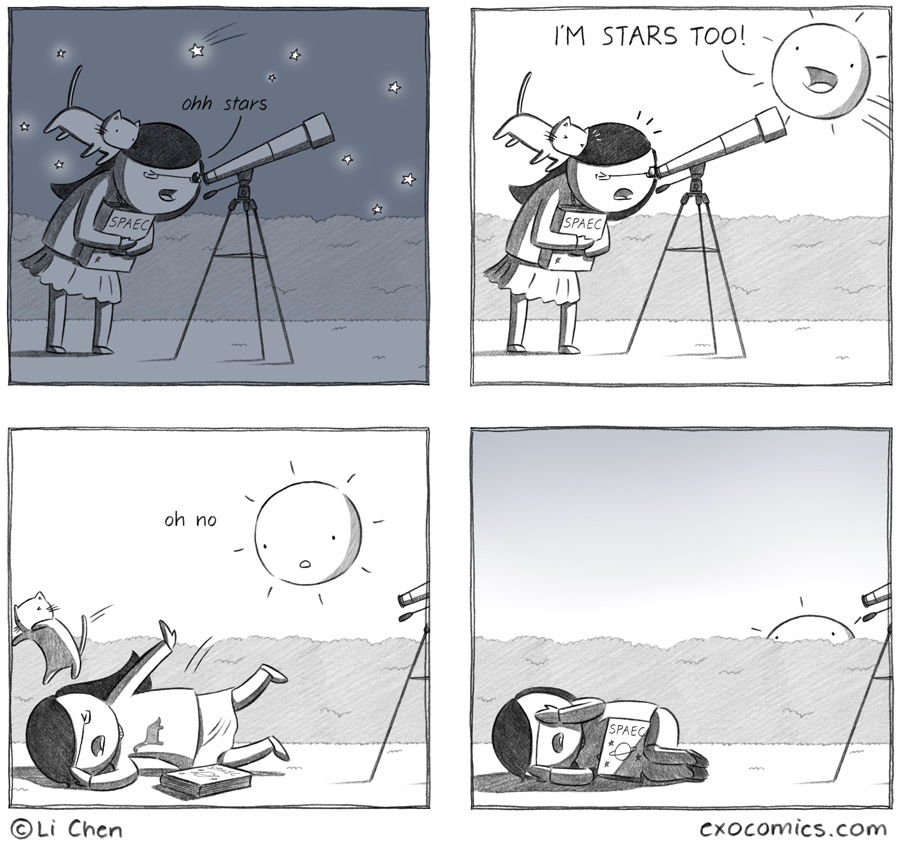
\includegraphics[height=.85\textheight,frame]{figs/comic.jpg}
    \end{figure}
\end{frame}

\appendix

\section{Appendix}

%\begin{frame}[fragile] \frametitle{Constructing Tagesstern}
%    \begin{figure}[!hb] 
%        \centering
%        \only<1>{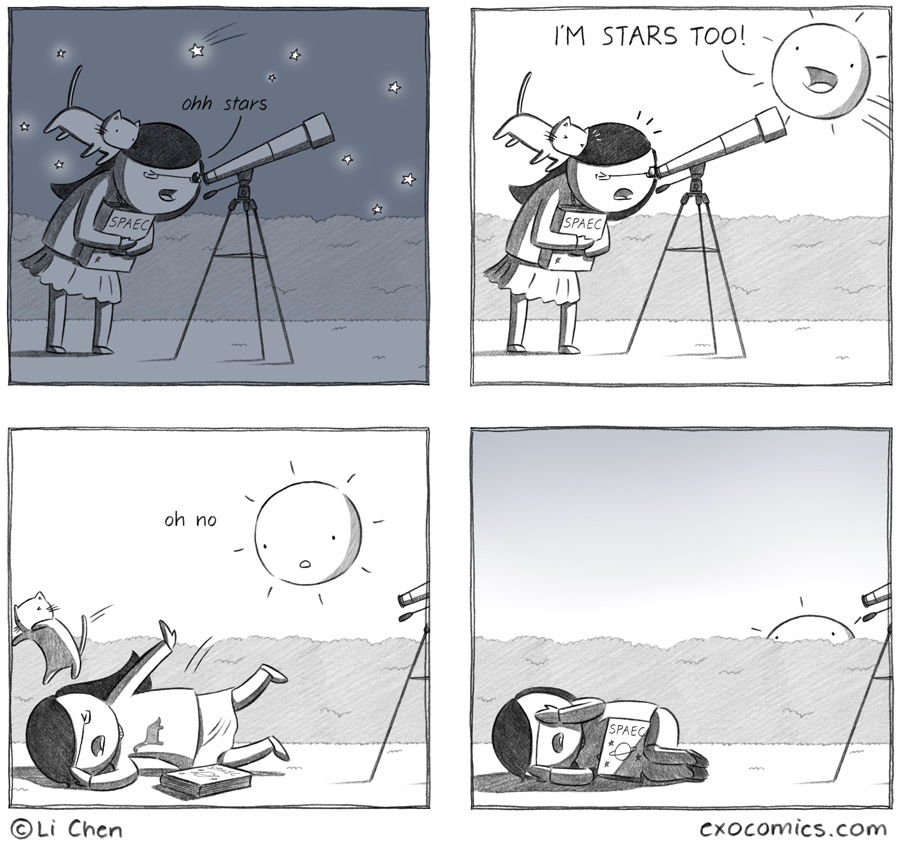
\includegraphics[height=.85\textheight,frame]{figs/comic.jpg}}
%        \only<2>{\includegraphics[height=.875\textheight, trim={0 0 2cm 0}, clip]{figs/tagesstern.pdf}}
%    \end{figure}
%\end{frame}

\begin{frame}[fragile] \frametitle{Initial points chosen}
    \begin{figure}[!hb] 
        \centering
        \includegraphics[width=\textwidth]{figs/inputs-slides.pdf}
    \end{figure}
\end{frame}

\begin{frame}[fragile] \frametitle{Model selection}
    \only<1>{
    \begin{equation}
      \vec B \equiv \qty[
        H_{\text{TAMS}}, 
        \ldots,
        %\min\qty(\vec H)+\frac{\max\qty(\vec H)-\min\qty(\vec H)}{99},
        \frac{(M-i)\cdot H_{\text{TAMS}}+H_{\text{ZAMS}}}{M-1}, 
        \ldots, 
        H_{\text{ZAMS}}
      ]
    \end{equation}
    \begin{equation}
      \boldsymbol C \equiv 
      \begin{bmatrix}
        \abs{B_1-H_1} & \abs{B_1-H_2} & \dots & \abs{B_1-H_N} \\ 
        \abs{B_2-H_1} & \abs{B_2-H_2} & \dots & \abs{B_2-H_N} \\ 
        \vdots & \vdots & \ddots & \vdots\\ 
        \abs{B_M-H_1} & \abs{B_M-H_2} & \dots & \abs{B_M-H_N}
      \end{bmatrix}
    \end{equation}}
    \only<2>{
    \begin{align}
      \hat{\boldsymbol{S}} = \underset{\boldsymbol S}{\arg\min} \; & \sum_{ij} S_{ij} C_{ij} \notag\\
      \text{subject to } & \sum_j S_{ij} \leq 1 \; \text{ for all } i=1\ldots N \notag\\
      \text{and } & \sum_i S_{ij} = 1 \; \text{ for all } j=1\ldots M.
    \end{align}}
    \begin{figure}[!hb] 
        \centering
        \only<1>{\includegraphics[width=\textwidth]{figs/spacing.png}}
        \only<2>{\includegraphics[width=\textwidth]{figs/spacing-ideal.png}}
    \end{figure}
\end{frame}

\begin{frame}[fragile] \frametitle{Principal components analysis}
    \begin{figure}[!hb] 
        \centering
        \includegraphics[height=.875\textheight, trim={0 0 2cm 0}, clip]{figs/corr-pca-slides.pdf}
        %\caption{Spearman correlation coefficients between model variables and principal components}
    \end{figure}
\end{frame}

\begin{frame}[fragile] \frametitle{Decision tree example}
    \begin{figure}[!hb] 
        \centering
        \input{figs/flowchart.tex}
    \end{figure}
\end{frame}

%\begin{frame}[fragile] \frametitle{Conclusions \& Future work}
%    \textbf{Summary}
%    \begin{itemize}
%        \item Studied the main sequence in five dimensions ($M$, $Y$, $Z$, $\alpha$, $\tau$)
%        \item 
%        \item 
%    \end{itemize}
    
%    \textbf{Future work}
%    \begin{itemize}
%        \item 
%        \item Structural inversions
%    \end{itemize}
%\end{frame}

\end{document}

